\documentclass[a4paper,11pt]{article} 
\usepackage{geometry}
\usepackage[italian,english]{babel}
\geometry{
    a4paper,
    total={170mm,257mm},
    left=20mm,
    top=20mm,
}
\usepackage{graphicx}
\usepackage{caption}
\usepackage{subcaption}
\usepackage{multirow}
\captionsetup{tableposition=bottom,figureposition=bottom}
\captionsetup[figure]{labelfont=bf,textfont=it}
\captionsetup[table]{labelfont=bf,textfont=it}

\begin{document}
\title{Analisi della caratteristica tensione corrente di un diodo}
\author{Giovanni Bugli \and Giovanni Postacchini}
\date{Novembre 2021, Postazione 11}

\maketitle
\begin{abstract}
  In questa esperienza di laboratorio è stata studiata la caratteristica tensione corrente per un diodo al germanio e per un diodo al silicio. Dalle misure effettuate è stato possibile stimare il prodotto $\eta V_T$, dove $\eta$ è  l'indice di idealità e $V_T$ la tensione termica,  e la corrente di saturazione $I_0$. I valori numerici stimati per il diodo al germanio e al silicio sono  rispettivamente: $\eta_{Ge} V_T = (43\pm 3) mV$, $\eta_{Si} V_T= (50\pm 4) mV$, $I_{0 Ge} = (2.6\pm 0.6) \mu A$, $I_{0 Si} = (2.0\pm 1.5) nA$ .
\end{abstract}
\selectlanguage{italian}
\section{Introduzione}
Lo scopo di questa prova è quello di studiare il comportamento di una giunzione pn polarizzata (diodo) analizzando i valori della corrente in funzione della tensione ai capi del diodo stesso. La caratteristica tensione-corrente di un diodo è espressa dall'equazione di Shockley:
\begin{equation}
  I_D = I_0 (e^{\frac{V_D}{\eta V_T}}-1)
\end{equation}
dove $I_D$ e $V_D$ sono rispettivamente la corrente e la tensione ai capi del diodo, $I_0$ la corrente di saturazione, $\eta$ il fattore di idealità e $V_T$ la tensione termica.

\section{Apparato sperimentale e svolgimento}
\begin{figure}[h!]
  \centering
  \includegraphics[width=0.7\linewidth]{schema_circuito.pdf}
  \caption{Schema del circuito realizzato. Sono rappresentati i terminali del generatore e del multimetro. In fase di misurazione, si è collegata la giunzione pn ai punti A e B.}
\end{figure}
Il circuito realizzato, come mostrato in Fig. 1, è formato dai seguenti componenti: un generatore di tensione costante da 5V, un potenziometro con fondoscala da 1$k\Omega$, una giunzione pn al germanio o al silicio. Per le misure di tensione si è utilizzato un oscilloscopio analogico GW modello GOS-652G mentre per quelle di corrente un multimetro digitale FLUKE modello 8022.
\newline
La risoluzione e la precisione specifiche del multimetro e dell'oscilloscopio relativi ai valori di fondo scala utilizzati nelle misure sono riportate in Tab 1. Le incertezze associate alle misure di tensione e corrente sono state calcolate come discusso in appendice.

\begin{table}[h!]
  \begin{center}
    \begin{tabular}{|c|c|c|c|}
      \hline
                                     & Fondo scala  & Risoluzione & Precisione                        \\
      \hline
      \multirow{4}{*}{Multimetro}    & $2 mA$       & $1\mu A$    & \multirow{2}{*}{0.75\% + 1 digit} \\
                                     & $20 mA$      & $10\mu A$   &                                   \\
      \cline{2-4}
                                     & $200 mV$     & $100 \mu V$ & \multirow{2}{*}{0.25\% + 1 digit} \\
                                     & $2 V$        & $1 mV$      &                                   \\
      \hline
      \multirow{5}{*}{Oscilloscopio} & $10 mV/div$  & $1 mV$      & \multirow{5}{*}{3\%}              \\
                                     & $20 mV/div$  & $2 mV$      &                                   \\
                                     & $50 mV/div$  & $5 mV$      &                                   \\
                                     & $100 mV/div$ & $10 mV$     &                                   \\
                                     & $200 mV/div$ & $20 mV$     &                                   \\
      \hline
    \end{tabular}
    \caption{Risoluzione e precisione degli strumenti di misura nei fondo scala utilizzati. La risoluzione dell'oscilloscopio è stata calcolata come fondoscala/10.}
  \end{center}
\end{table}

I componenti sono stati montati su una scheda millepori alla quale sono stati collegati opportunamente anche il generatore di tensione e gli strumenti di misura quali il multimetro e l'oscilloscopio.
In un primo momento è stato tolto il diodo dal circuito ed è stata verificata la corretta calibrazione tra i due strumenti nel misurare i valori di tensione. Sono state effettuate così una serie di misure di tensione, riportate in Tab. 2, che hanno confermato l'assenza di errori sistematici nella misura della tensione tra l'oscilloscopio e il multimetro. Infatti, come mostrato in Fig. 2,  è stato eseguito un fit attraverso la relazione lineare $V_{oscilloscopio} = A + B V_{multimetro}$, ottenendo le seguenti stime per i parametri: $A = (1 \pm 2) mV$ , $B = (0.972 \pm 0.016)$. I prarametri stimati, sono compatibili, entro $2\sigma$, ai valori attesi $A = 0 mV$ e $B=1$.

\begin{table}[h!]
  \begin{center}
    \begin{tabular}{c|c|c|c}
      \textbf{$V_{multimetro}$(mV)} & \textbf{Fscala (mV)} & \textbf{$V_{oscilloscopio}$ (mV)} & \textbf{Fscala (mV/div)} \\
      \hline
      $50.1 \pm 0.2 $               & 200                  & $50 \pm 2 $                       & $10$                     \\
      $102.9 \pm 0.4 $              & 200                  & $100 \pm 4 $                      & $20$                     \\
      $157.8 \pm 0.5 $              & 200                  & $150 \pm 7 $                      & $50$                     \\
      $208 \pm 2 $                  & 2000                 & $200 \pm 8 $                      & $50$                     \\
      $256 \pm 2 $                  & 2000                 & $250 \pm 9 $                      & $50$                     \\
      $306 \pm 2 $                  & 2000                 & $300 \pm 10 $                     & $50$                     \\
      $361 \pm 2 $                  & 2000                 & $350 \pm 15 $                     & $100$                    \\
      $410 \pm 2$                   & 2000                 & $400 \pm 16 $                     & $100$                    \\
      $461 \pm 2$                   & 2000                 & $450 \pm 17 $                     & $100$                    \\
      $509 \pm 2$                   & 2000                 & $500 \pm 18 $                     & $100$                    \\
      $560 \pm 2$                   & 2000                 & $550 \pm 19 $                     & $100$                    \\
    \end{tabular}
    \caption{Tensione misurata ai capi del multimetro e dell'oscilloscopio. Accanto ad ogni dato è riportato il valore di fondo scala adoperato in fase di misurazione.}
  \end{center}
\end{table}

\begin{figure} [h!]
  \centering
  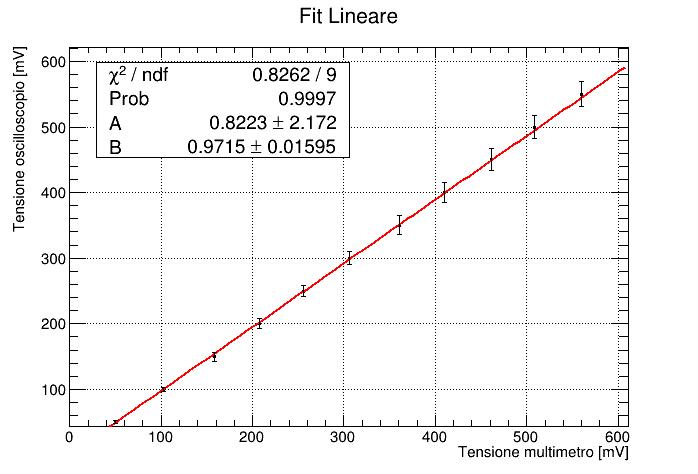
\includegraphics[width=0.7\linewidth]{../analisi dati/calibrazione.png}
  \caption{Retta di calibrazione per verificare l'assenza di errori sistematici nelle misure di tensione tra il multimetro e l'oscilloscopio. La linea rossa raffigura il fit lineare eseguito sui punti misurati.}
\end{figure}


Successivamente è stato montato prima il diodo al germanio e poi quello al silicio in polarizzazione diretta e sono state effettuate misure di corrente e di tensione variando la resistenza del potenziometro. Le misure sono state effetuate in un range di tensioni da 50 a 800 mV circa, in modo tale da sottopore i diodi ad una corrente non superiore a 1 - 2 mA.
\newpage
\section{Risultati e discussione}
I dati sperimentali relativi alla tensione e alla corrente presenti nel diodo sono visibili in Tab 3(Ge) e Tab 4(Si).

\begin{table}[h!]
  \begin{center}
    \begin{tabular}{c|c|c|c}
      \textbf{$V_{Ge}$ (mV)}    & \textbf{Fscala (mV/div)} & \textbf{$I_{Ge}$ (mA)} & \textbf{Fscala (mA)} \\
      \hline
      $50 \pm 5$                & 50                       & $0.005 \pm 0.001$      & 2                    \\
      $60 \pm 5$                & 50                       & $0.008 \pm 0.001$      & 2                    \\
      $70 \pm 5$                & 50                       & $0.010 \pm 0.001$      & 2                    \\
      $75 \pm 5$                & 50                       & $0.012 \pm 0.001$      & 2                    \\
      $80 \pm 6$                & 50                       & $0.014 \pm 0.001$      & 2                    \\
      $90 \pm 6$                & 50                       & $0.018 \pm 0.001$      & 2                    \\
      $100 \pm 6$               & 50                       & $0.025 \pm 0.001$      & 2                    \\
      $110 \pm 6$               & 50                       & $0.032 \pm 0.001$      & 2                    \\
      $120 \pm 6$               & 50                       & $0.042 \pm 0.001$      & 2                    \\
      $125 \pm 6$               & 50                       & $0.046 \pm 0.001$      & 2                    \\
      $130 \pm 6$               & 50                       & $0.054 \pm 0.001$      & 2                    \\
      $140 \pm 7$               & 50                       & $0.066 \pm 0.001$      & 2                    \\
      $150 \pm 7$               & 50                       & $0.084 \pm 0.002$      & 2                    \\
      $160 \pm 7$               & 50                       & $0.101 \pm 0.002$      & 2                    \\
      $170 \pm 7$               & 50                       & $0.126 \pm 0.002$      & 2                    \\
      $175 \pm 7$               & 50                       & $0.140 \pm 0.002$      & 2                    \\
      $180 \pm 7$               & 50                       & $0.152 \pm 0.002$      & 2                    \\
      $190 \pm 8$               & 50                       & $0.189 \pm 0.002$      & 2                    \\
      $200 \pm 8$               & 50                       & $0.234 \pm 0.003$      & 2                    \\
      $225 \pm 8$               & 50                       & $0.359 \pm 0.004$      & 2                    \\
      $250 \pm 9$               & 50                       & $0.585 \pm 0.005$      & 2                    \\
      $(27.5 \pm 1.0) \cdot 10$ & 50                       & $0.890 \pm 0.008$      & 2                    \\
      $(30.0 \pm 1.0) \cdot 10$ & 50                       & $1.362 \pm 0.011$      & 2                    \\
    \end{tabular}
    \caption{Tensione misurata con l'oscilloscopio e corrente misurata dal multimetro per il diodo al germanio. Accanto ad ogni dato è riportato il valore di fondo scala adoperato in fase di misurazione.}
  \end{center}
\end{table}

\begin{table}[h!]
  \begin{center}
    \begin{tabular}{c|c|c|c}
      \textbf{$V_{Si}$ (mV)}    & \textbf{Fscala (mV/div)} & \textbf{$I_{Si}$ (mA)} & \textbf{Fscala (mA)} \\
      \hline
      $(40.0 \pm 1.6) \cdot 10$ & 100                      & $0.006 \pm 0.001$      & 2                    \\
      $(42.0 \pm 1.6) \cdot 10$ & 100                      & $0.008 \pm 0.001$      & 2                    \\
      $(44.0 \pm 1.7) \cdot 10$ & 100                      & $0.013 \pm 0.001$      & 2                    \\
      $(46.0 \pm 1.7) \cdot 10$ & 100                      & $0.019 \pm 0.001$      & 2                    \\
      $(48.0 \pm 1.8) \cdot 10$ & 100                      & $0.030 \pm 0.001$      & 2                    \\
      $(50.0 \pm 1.8) \cdot 10$ & 100                      & $0.042 \pm 0.001$      & 2                    \\
      $(52.0 \pm 1.9) \cdot 10$ & 100                      & $0.069 \pm 0.001$      & 2                    \\
      $(54.0 \pm 1.9) \cdot 10$ & 100                      & $0.101 \pm 0.001$      & 2                    \\
      $(56 \pm 2) \cdot 10$     & 100                      & $0.159 \pm 0.001$      & 2                    \\
      $(58 \pm 2) \cdot 10$     & 100                      & $0.241\pm 0.002$       & 2                    \\
      $(60 \pm 2) \cdot 10$     & 100                      & $0.375\pm 0.002$       & 2                    \\
      $(64 \pm 3) \cdot 10$     & 200                      & $0.611 \pm 0.003$      & 2                    \\
      $(72 \pm 3) \cdot 10$     & 200                      & $2.020 \pm 0.015$      & 20                   \\
      $(76 \pm 3) \cdot 10$     & 200                      & $5.72 \pm 0.02$        & 20                   \\
    \end{tabular}
    \caption{Tensione misurata con l'oscilloscopio e corrente misurata dal multimetro per il diodo al silicio. Accanto ad ogni dato è riportato il valore di fondo scala adoperato in fase di misurazione.}
  \end{center}
\end{table}

In Fig 3 sono graficati i punti sperimentali acquisiti sia per il diodo al germanio sia per quello al silicio. Sono ben visibili i due diversi valori di tensione di soglia, pari a $V_\gamma \simeq 50 mV $ per il germanio e $V_\gamma \simeq 400 mV $ per il silicio.


\begin{figure} [h!]
  \centering
  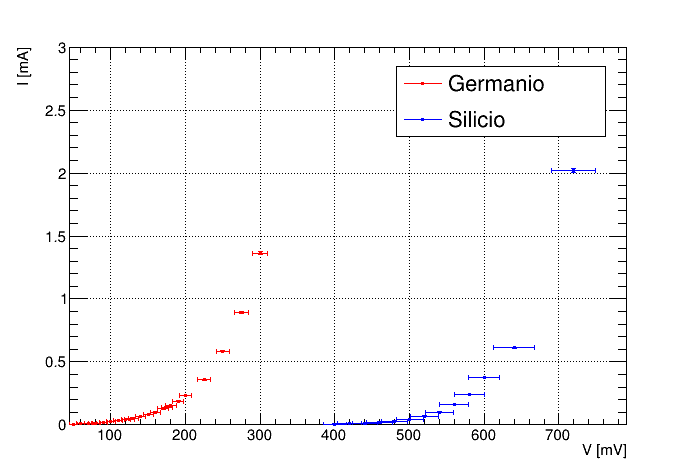
\includegraphics[width=0.7\linewidth]{../analisi dati/caratteristiche _dati.png}
  \caption{Caratteristica tensione-corrente dei diodi al germanio e al silicio osservata in polarizzazione diretta. Il grafico è stato ottenuto sovrapponendo i dati sperimentali osservati separatamente per i due diodi}
\end{figure}

Sui dati di tensione e corrente è stato eseguito un fit con l'Eq. 1. In Fig. 4 vengono rappresentate le curve caratteristiche in scala semilogaritmica per i due diodi.

\begin{figure} [h]
  \begin{subfigure}{0.49\textwidth}
    \centering
    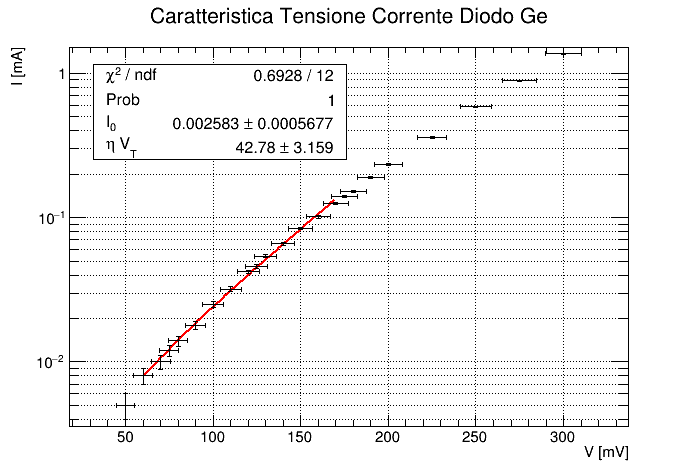
\includegraphics[width = \textwidth]{../analisi dati/germanio_fit.png}
  \end{subfigure}
  \begin{subfigure}{0.49\textwidth}
    \centering
    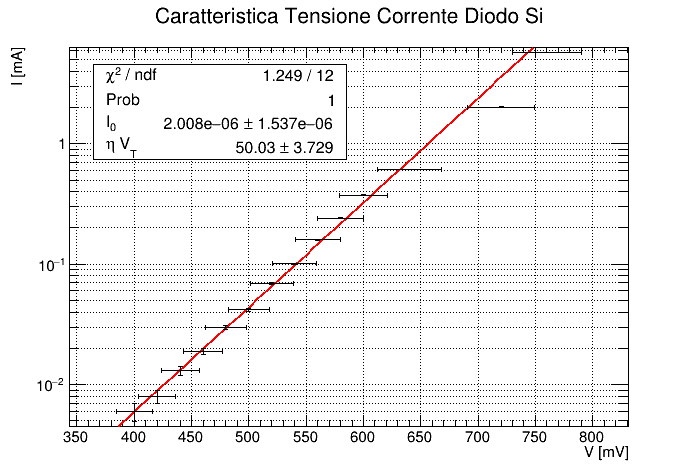
\includegraphics[width = \textwidth]{../analisi dati/silicio_fit.png}
  \end{subfigure}
  \caption{Caratteristica tensione-corrente dei diodi in polarizzazione diretta. I dati sono rappresentati in scala semilogaritmica. Il dati sono stati fittati attraverso l'equazione di Schockley. I parametri ottenuti dal fit sono riportati nei grafici.}
\end{figure}

In particolare per il germanio il fit è stato eseguito in un range ridotto di 60-170 mV poichè a tensioni maggiori il comportamento lineare in scala semilogaritmica non è ottimale, mentre per il diodo al silcio si è fittato in un range di 400 - 760 mV su tutti i dati acquisiti. In entrambi i casi il fit ha prodotto un buon $\tilde{\chi}^2$ che permette di giustificare la validità dei parametri ottenuti. Numericamete $\tilde{\chi}_{Ge} \simeq 0.06 $ , $\tilde{\chi}_{Si} \simeq 0.1 $ che risultano inferiori valore ottimale $\tilde{\chi}^2 \simeq 1 $. Il motivo di tale disaccordo si giustifica con l'elevato errore relativo associato alle misure di tensione esegute con l'oscilloscopio.
Come riportato in Fig. 4, i parametri caratteristici ricavati dal fit sono: $\eta_{Ge} V_T = (43\pm 3) mV$, $\eta_{Si} V_T= (50\pm 4) mV$, $I_{0 Ge} = (2.6\pm 0.6) \mu A$, $I_{0 Si} = (2.0\pm 1.5) nA$.

Supponendo i diodi ad una temperatura pari alla temperatura ambiente $T= 300K$, possiamo supporre $V_T \simeq 26 mV$ e ricavare indirettamente l'indice di idealità dalle stime di $\eta V_T$: $\eta_{Ge} = (1.65 \pm 0.11) $ ,  $\eta_{Si} = (1.92 \pm 0.15) $. Questi parametri sono solo indicativi in quanto non è stata misurata la temperatura effettiva dei diodi né tantomento è stato verificato che il valore riusultasse costante durante le misure.

\section{Conclusioni}
L'esperimento effettuato in laboratorio ha confermato l'andamento esponenziale della corrente previsto dall'equazione di Schockley sia per il diodo al silicio che per quello al germanio.
Infatti, le operazioni di best-fitting sui dati acquisiti hanno mostrato la compabilità con l'andamento atteso dalla equazione di Schockley (Eq. 1). Dagli stessi fits, si sono ricavati i parametri caratteristici relativi ai due diodi: $\eta_{Ge} V_T = (43\pm 3) mV$, $\eta_{Si} V_T= (50\pm 4) mV$, $I_{0 Ge} = (2.6\pm 0.6) \mu A$, $I_{0 Si} = (2.0\pm 1.5) nA$ .

\section*{Appendice: stima delle incetezze}
L'incertezza sulle misure di corrente effettuate con il multimetro è 0.75\% della lettura + 1 digit. L'incertezza sulle misure di tensione effettuate con l'oscilloscopio $\sigma_{osc}$ è stata calcolata sommando in quadratura l'errore sulla lettura $\sigma_L$, l'errore sullo zero $\sigma_Z$ e l'errore del costruttore $\sigma_C$ secondo la formula:
\begin{equation}
  \sigma_{osc} = \sqrt{\sigma_{L}^2+ \sigma_{Z}^2+ \sigma_{C}^2}
\end{equation}
dove l'errore sulla lettura è $fondo scala / 10$ mentre $\sigma_{C}$ corrisponde al 3\% della lettura.


\end{document}